% Generated 2021-08-25 18:02:23 +0530
\subsection{References} \label{sec:References}


\block{References} \glspl{organize} \block{Reference} elements.

\block{References} may be modeled as part of a \block{Device}, \block{Component} or \block{Interface} type \gls{structural element}.

\begin{figure}[ht]
  \centering
    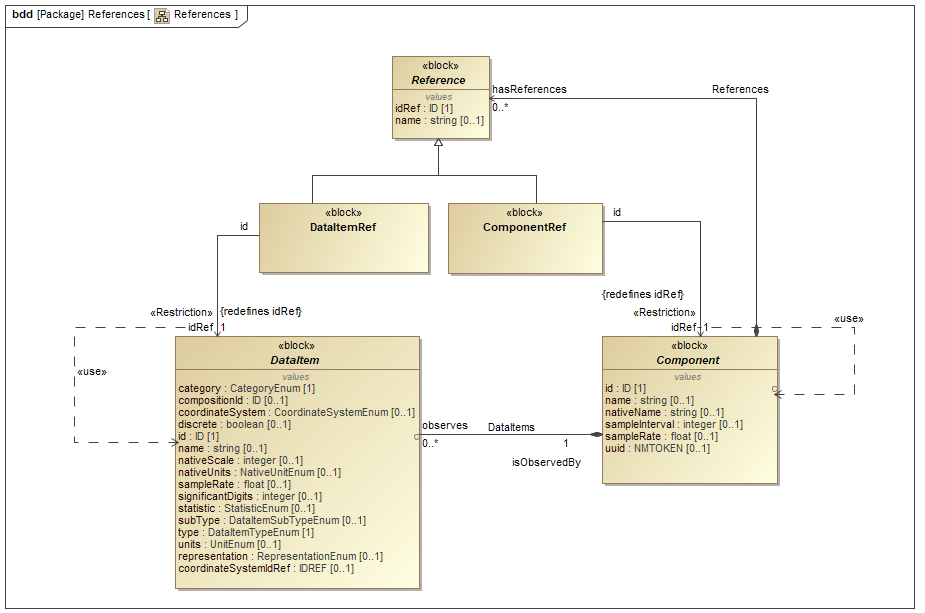
\includegraphics[width=1.0\textwidth]{figures/References.png}
  \caption{References Diagram}
  \label{fig:References Diagram}
\end{figure}

\FloatBarrier


Note: See \sect{References Schema Diagrams} for XML schema of \block{Reference} and its types.


\subsubsection{Reference}
\label{sec:Reference}



\block{Reference} is a pointer to information that is associated with another \gls{structural element} defined elsewhere for a piece of equipment.


\paragraph{Attributes of Reference}\mbox{}
\label{sec:Attributes of Reference}

\tbl{Attributes of Reference} lists the attributes of \texttt{Reference}.

\begin{table}[ht]
\centering 
  \caption{Attributes of Reference}
  \label{table:Attributes of Reference}
\tabulinesep=3pt
\begin{tabu} to 6in {|l|l|l|} \everyrow{\hline}
\hline
\rowfont\bfseries {Attribute} & {Type} & {Multiplicity} \\
\tabucline[1.5pt]{}

\property{idRef}[Reference] & \texttt{IDREF} & 1 \\
\property{name}[Reference] & \texttt{string} & 0..1 \\
\end{tabu}
\end{table}
\FloatBarrier

Descriptions for attributes of \block{Reference}:

\begin{itemize}

\item \property{idRef}[Reference] \newline A pointer to the \block{id} attribute of an element that contains the information to be associated with this XML element.

\item \property{name}[Reference] \newline The name of an element or a piece of equipment.
\end{itemize}



\subsubsection{DataItemRef}
\label{sec:DataItemRef}



\block{DataItemRef} is a pointer to a \gls{data entity} associated with another \gls{structural element} defined for a piece of equipment.  \block{DataItemRef} allows the data associated with a data item defined in another \gls{structural element} to be directly associated with this element.


\paragraph{Attributes of DataItemRef}\mbox{}
\label{sec:Attributes of DataItemRef}

\tbl{Attributes of DataItemRef} lists the attributes of \texttt{DataItemRef}.

\begin{table}[ht]
\centering 
  \caption{Attributes of DataItemRef}
  \label{table:Attributes of DataItemRef}
\tabulinesep=3pt
\begin{tabu} to 6in {|l|l|l|} \everyrow{\hline}
\hline
\rowfont\bfseries {Attribute} & {Type} & {Multiplicity} \\
\tabucline[1.5pt]{}

\property{idRef}[DataItemRef] & \texttt{DataItem} & 1 \\
\end{tabu}
\end{table}
\FloatBarrier

Descriptions for attributes of \block{DataItemRef}:

\begin{itemize}

\item \property{idRef}[DataItemRef] \newline A pointer to the \property{id} attribute of the \block{DataItem} that contains the information to be associated with this element.
\end{itemize}



\subsubsection{ComponentRef}
\label{sec:ComponentRef}



\block{ComponentRef} is a pointer to all of the information associated with another \gls{structural element} defined for a piece of equipment.  \block{ComponentRef} allows all of the information (\gls{Lower Level} \block{Components} and all \glspl{data entity}) that is associated with the other \gls{structural element} to be directly associated with this element.


\paragraph{Attributes of ComponentRef}\mbox{}
\label{sec:Attributes of ComponentRef}

\tbl{Attributes of ComponentRef} lists the attributes of \texttt{ComponentRef}.

\begin{table}[ht]
\centering 
  \caption{Attributes of ComponentRef}
  \label{table:Attributes of ComponentRef}
\tabulinesep=3pt
\begin{tabu} to 6in {|l|l|l|} \everyrow{\hline}
\hline
\rowfont\bfseries {Attribute} & {Type} & {Multiplicity} \\
\tabucline[1.5pt]{}

\property{idRef}[ComponentRef] & \texttt{Component} & 1 \\
\end{tabu}
\end{table}
\FloatBarrier

Descriptions for attributes of \block{ComponentRef}:

\begin{itemize}

\item \property{idRef}[ComponentRef] \newline A pointer to the \property{id} attribute of the \block{Component} that contains the information to be associated with this element.
\end{itemize}


